\documentclass[usletter]{article}
\usepackage{graphicx}
\usepackage{amsfonts}
\usepackage{amsthm}
\usepackage{amsmath}
\usepackage{scribe}
\usepackage[margin=1.5in]{geometry}
\usepackage{algorithm}
\usepackage{algorithmicx}
\usepackage{float}
\usepackage[noend]{algpseudocode}

\begin{document}

\makeheader{Minsheng Zhang}                              % your name
           {April 26, 2015}                          % lecture date
           {14}                                       % lecture number
           {Approximation algorithm}  % lecture title

\noindent
In this week, we talked about three different problems. They are max set, feedback vertex set problem in undirected graph and shortest s-t path problem. We mainly talked about how to solve these problems using primal-dual method.

\section{Max Set}
In the maximum satisfiability problem (often abbreviated as MAX SAT), the input consists of n Boolean variables $x_1$, . . . , $x_n$ (each of which may be set to either true or false), m clauses $C_1$,...,$C_m$ (each of which consists of adisjunction (that is, an “or”) of some number of the variables and their negations – for example, $x_3$ $\vee$ $\overline{x_5}$ $\vee$ $x_{11}$, where  $\overline{x_i}$ is the negation of $x_i$), and a nonnegative weight $w_j$ for each clause $C_j$. The objective of the problem is to find an assignment of true/false to the $x_i$ that maximizes the weight of the satisfied clauses. This problem is a NP-hard problem.\\


First we define some concepts:
\begin{enumerate}
	\item $x_i$ positive literal, $\overline{x_i}$ negative literal. 
	\item $L_j$: number of literals in the clause $C_j$; if $L_j$ = 1, $C_j$ is a "unit".
\end{enumerate}

Claim: setting each $x_i$ to true with probablity 1/2 independently gives us a randomized 1/2-approximation algo. \\

Define $y_j$ = $\left\{
\begin{array}{c}
1 \quad if \quad C_j \quad satisfied\\
0 \quad o.w.\\
\end{array}
\right.$

Then the the weight of the satisfied clauses W = $\sum_{j=1}^m y_j*w_j$. We can evaluate its expectation as: \\ E[W] = $\sum_{j=1}^m w_j*E[y_j]$. Since we set each $x_i$ to true with probablity 1/2 independently, E[$y_j$] = Pr($C_j$ is satisfied) = $\sum V_i * P(y_j = V_i)$ = 1*1/2 + 0*1/2 = 1/2. \\ Now let computer the probality that one clause is satisfied. We can easily get it from the probality that one clause is not satisfied with 1-P($y_j$=0). And P($y_j$=0) = P(Postive Lietrals = False and Negative Literals = true) = ${(1/2)}^{L_j}$. Then P($y_j$=1) = 1-${(1/2)}^{L_j}$ $\ge$ 1/2. Continue with the expectation: \\
E[W] $\ge$ 1/2 $\sum_{j=1}^m {w_j}$ $\ge$ 1/2 OPT. And $\sum_{j=1}^m {w_j}$ is a upper bound of OPT. Even the expectation value is greater than 1/2 OPT, you cannot garantee that every time your randomization can get a such result, we will introduce you a derandomize method later.\\
Derandomization: derandomize a randomized algorithm is to obtain a deterministic algorithm whose solution value is as good as the expected value of the randomized algorithm. \\
More formally, if E [W |$x_1$ $\leftarrow$ true] ≥ E [W |$x_1$ $\leftarrow$ false], then we set $x_1$ true, otherwise we set it to false. Since by the definition of conditional expectations, \\

E[W ] = E[W |$x_1$ $\leftarrow$ true] Pr[$x_1$ $\leftarrow$ true] + E[W |$x_1$ $\leftarrow$ false] Pr[$x_1$ $\leftarrow$ false] = 1 (E[W|$x_1$ $\leftarrow$ true] + E[W|$x_1$ $\leftarrow$ false]),\\
if we set $x_1$ to truth value $b_1$ so as to maximize the conditional expectation, then E[W|$x_1$ $\leftarrow$ $b_1$] ≥ E[W]; that is, the deterministic choice of how to set $x_1$ guarantees an expected value no less than the expected value of the completely randomized algorithm.


\section{Dual Approximation Algorithm for Feedback vertex set problem in undirected graph}
After that, we talked about the feed back vertex set problem in undirected graph. Given a graph G(V,E) and for every vertex there is a weight W.
We want to find a set of vertices S so that the graph G(V-S) contains no cycle. After find S we calculate the weights of vertices in it. The problem is to minimize $\sum_{i \in S} {W_i}$.

For example we are given a graph G in Figure~\ref{fig:FVS}. The weights W for the vertices are 2, 3, 4, 5 respectively. There are three cycles, V1-V2-V3, V1-V2-V4, V1-V4-V2-V3. For example, we can choose set$ {V3, V4}$. So that the new graph only contains ${V1, V2}$ which has no cycle, the sum of V3 and V4 is 9. But here in this example, the optimal solution is $S={V1}$ with weight 2.

\begin{figure}[bht]
\begin{center}
     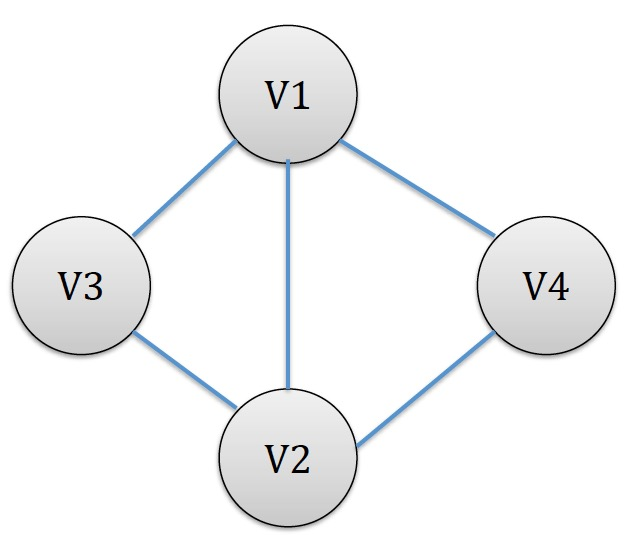
\includegraphics[width=3.0in]{figures/FVS}
\caption{\label{fig:FVS}feed back vertex set problem in undirected graph}
\end{center}
\end{figure}

After that we show we can convert this problem to Integer programming. For every vertex v, we use $ X_i = {0, 1}$ to denote whether the vertex is in the set S or not. Then we let C denote the set of all cycles c in the graph, we can formulate the feedback vertex set problem in undirected graphs as the following integer program: $\min{\sum_{i \in S} {W_i}}$ and the constraint is: $\sum_{i \in C} X_i \ge 1$.

If we relax the integer program to a linear program by replacing the constraints $xi \in \{0, 1\}$ with $xi \ge 0$, and take its dual, we obtain the dual is to $\max{\sum_{c \in C} y}$ and the constraint is: $\sum_{c \in C; i \in c} y \le W_I$

By analogy with the primal-dual algorithm for the set-cover problem, we get the greedy algorithm to solve the problem. We start with the dual feasible solution in which all y are set to zero, and with the primal infeasible solution $S = \emptyset$.

\begin{algorithm}
\caption{Greedy FVS in undirected graph}
\begin{algorithmic}[1]
\State y $\leftarrow$ 0
\State S $\leftarrow$  $\emptyset$
\While {there exists a cycle C in Gs} 
	\State Increase y until there is some l $\in$ C such that  $\sum_{c \in C; i \in c} y = W_l$
	\State S $\leftarrow$ S $\cup$ $\{l\}$
	\State Repeatedly remove vertices from graph with degree one from G
\State return S
\EndWhile
\end{algorithmic}
\end{algorithm}

Then we analysis the algorithm the same as it is for the set cover problem. Let S be the final set of vertices chosen. Thus we can write $\sum_{i \in S}{W_i} = \sum_{i \in S}{\sum_{i \in C}{y}}= \sum_{c \in C}{|S \cap c| y}$. So if $|S \cap c| \le \alpha$. We can say the $\sum_{i \in S}{W_i} \le \alpha * OPT$. After that, we prove that if we carefully choose y to increase, we can find a $4log_2{n}$ approximation algorithm.

First, for any path P of vertices of degree two in graph G, the greedy algorithm will choose at most one vertex from P; that is, $|S \cap P| \le$  1 for the final solution S given by the algorithm.

After that we prove that, in any graph G that has no vertices of degree one, there is a cycle with at most 2$log_2{n}$ vertices of degree three or more, and it can be found in linear time, because the depth of the BFS search tree is $log_2{n}$. By oberservation, each path of vertices of degree two joining two vertices of degree three or more in C can contain at most one vertex of S. Thus if C has at most $2log_2{n}$ vertices of degree three or more, it can have at most 4$log_2{n}$ vertices of S overall. So we can get a $4log_2{n}$ approximation algorithm.

\section{Dual approximation algorithm for shortest s-t path problem}
In the shortest s-t path problem, we are given an undirected graph G = (V,E), nonnegative costs $C_e$ ≥ 0 on all edges e $\in$ E, and a pair of distinguished vertices s and t. The goal of this problem is to find the minimum-cost path from s to t.  It is well-known that this problem is a P problem. For instance, we can solve this problem using Dijkstra's Algorithm. And here, the primal-dual method turns out to be equivalent to Dijkstra's Algorithm.

First we introduce the definition for set of s-t cut that is  $s \subset V; s \in S,t \notin s$.We use set S to denote all the s-t cuts.  And we use $\delta(S)$ to denote the set of all edges that have one endpoint in S and the other endpoint not in S. Then we can covert this problem to Integer Programming. The objection is $\min{\sum_{e \in E}{C_e*X_e}}$ and the constraint is $\sum_{e \in \delta(S)} \ge 1$.

Then the same as the feedback vertex set problem. We will find the dual of the Integer Programming version.
The objective function is $\sum_{s \in S}{y}$ and the constraint is $\sum{y} \le C_e$.

Then still we solve this problem by increasing variable Y(greedy). So that we get the algorithm:
\begin{algorithm}
\caption{Dual algorithm for the shortest s-t path problem.}
\begin{algorithmic}[1]
\State y $\leftarrow$ 0
\State F $\leftarrow$ $\emptyset$
\While {there is no s-t path in (V, F)}
	\State  Let C be the connected compoent of (V, F) containing s
	\State Increase $y_C$ until there is an edge e' $\in$ $\delta{C}$ such that $\sum_{S \in S:e' \in \delta{S} y_S}$ = $c_{e'}$
	\State F $\leftarrow$ F $\cup$ \{e'\}
\EndWhile
\State Let P be an s-t path in (V, F) 
\State \Return P
\end{algorithmic}
\end{algorithm}

Then we analysis the algorithm the same as it is for the FVS problem. Let P be the final path chosen. Thus we can write $\sum_{e \in P}{C_e} = \sum_{s \in S; t \notin S}{|P \cap \delta(S)| y}$.  SO next we show that $|P \cap \delta(S)|$ is equal to 1. Then we can say that $\sum_{e \in P}{C_e} \le OPT$.

We now show that if y > 0, then $|P \cap \delta(S)|$ = 1. Suppose otherwise, and$|P \cap \delta(S)|$  > 1. Then there must be a subpath P′ of P joining two vertices of S such that the only vertices of P ′ in S are its start and end vertices. Thus there is a cycle in the path P that it travels to S part and T part which is not a shortest path solution. Thus we have $|P \cap \delta(S)|$  = 1.

\bibliographystyle{abbrv}
\bibliography{0426}

\end{document}
